\documentclass[ucs,9pt]{beamer}
% \documentclass[ucs,9pt,handout]{beamer}
\setbeamercovered{transparent}
\newcommand{\semitransp}[2][35]{\color{fg!#1}#2}

\usepackage[utf8x]{inputenc} % Set input encoding to UTF-8.
\usepackage[english]{babel} % Set language.
\usepackage{nicefrac}
\usepackage{courier}

% activate KDE theme
\usepackage{KDE/beamerthemeKDE}
\usepackage{tikz}
\usepackage{multicol}
\usepackage{listings}

\title[Device Tailored Wayland Compositors]{Device Tailored Compositors}
\subtitle{with the QtWayland-Compositor Framework}
\author{Andreas Cord-Landwehr}
\date{\textnormal{February 5, 2017\\[\medskipamount] FOSDEM, Brussels}}

\newcommand{\KDEemail}{cordlandwehr@kde.org}
% % % \newcommand{\KDEweb}{https://talks.cord-landwehr.de}
% % % \newcommand{\KDEaffiliation}{KDE Developer}
% % %

\lstset{ %
  language=C++,
  backgroundcolor=\color{KDEgray4},
  basicstyle=\footnotesize\ttfamily,
  breakatwhitespace=false,
  breaklines=true,
  captionpos=b,
  commentstyle=\color{KDEgreen},
  escapeinside={\%*}{*)},
  extendedchars=true,
  frame=single,
  keywordstyle=\color{KDEblue},
  language=Prolog,
  numbers=left,
  numbersep=5pt,
  numberstyle=\tiny\color{lightgray},
  rulecolor=\color{lightgray},
  showspaces=false,
  showstringspaces=false,
  showtabs=false,
  stepnumber=1,
  stringstyle=\color{KDEorange},
  tabsize=2,
  title=\lstname,
  morekeywords={Item,import,not,\},\{,Q_SIGNALS,public,Q_OBJECT,virtual,NOTIFY,Q_NULLPTR,Q_DISABLE_COPY,Q_DECL_OVERRIDE},
  deletekeywords={time}
}

%TikZ Definitions
\usetikzlibrary{arrows}
\usetikzlibrary{fit}
\usetikzlibrary{shadows}
\usetikzlibrary{patterns}
\usetikzlibrary{matrix}
\usetikzlibrary{shapes}
\usetikzlibrary{calc}
\usetikzlibrary{decorations.pathmorphing}
\usetikzlibrary{positioning}
\usetikzlibrary{backgrounds}
\usetikzlibrary{decorations}
\usetikzlibrary{decorations.pathreplacing}

\usepackage[variablett]{lmodern}

\newcommand*{\eswap}[3]{#1:[#2\rightarrow#3]}

\begin{document}
\maketitle

\begin{frame}
    {Introduction}
    {About Me \& the Talk}

    \begin{textblock*}{.4\paperwidth}[1,0](\paperwidth,0pt)%
        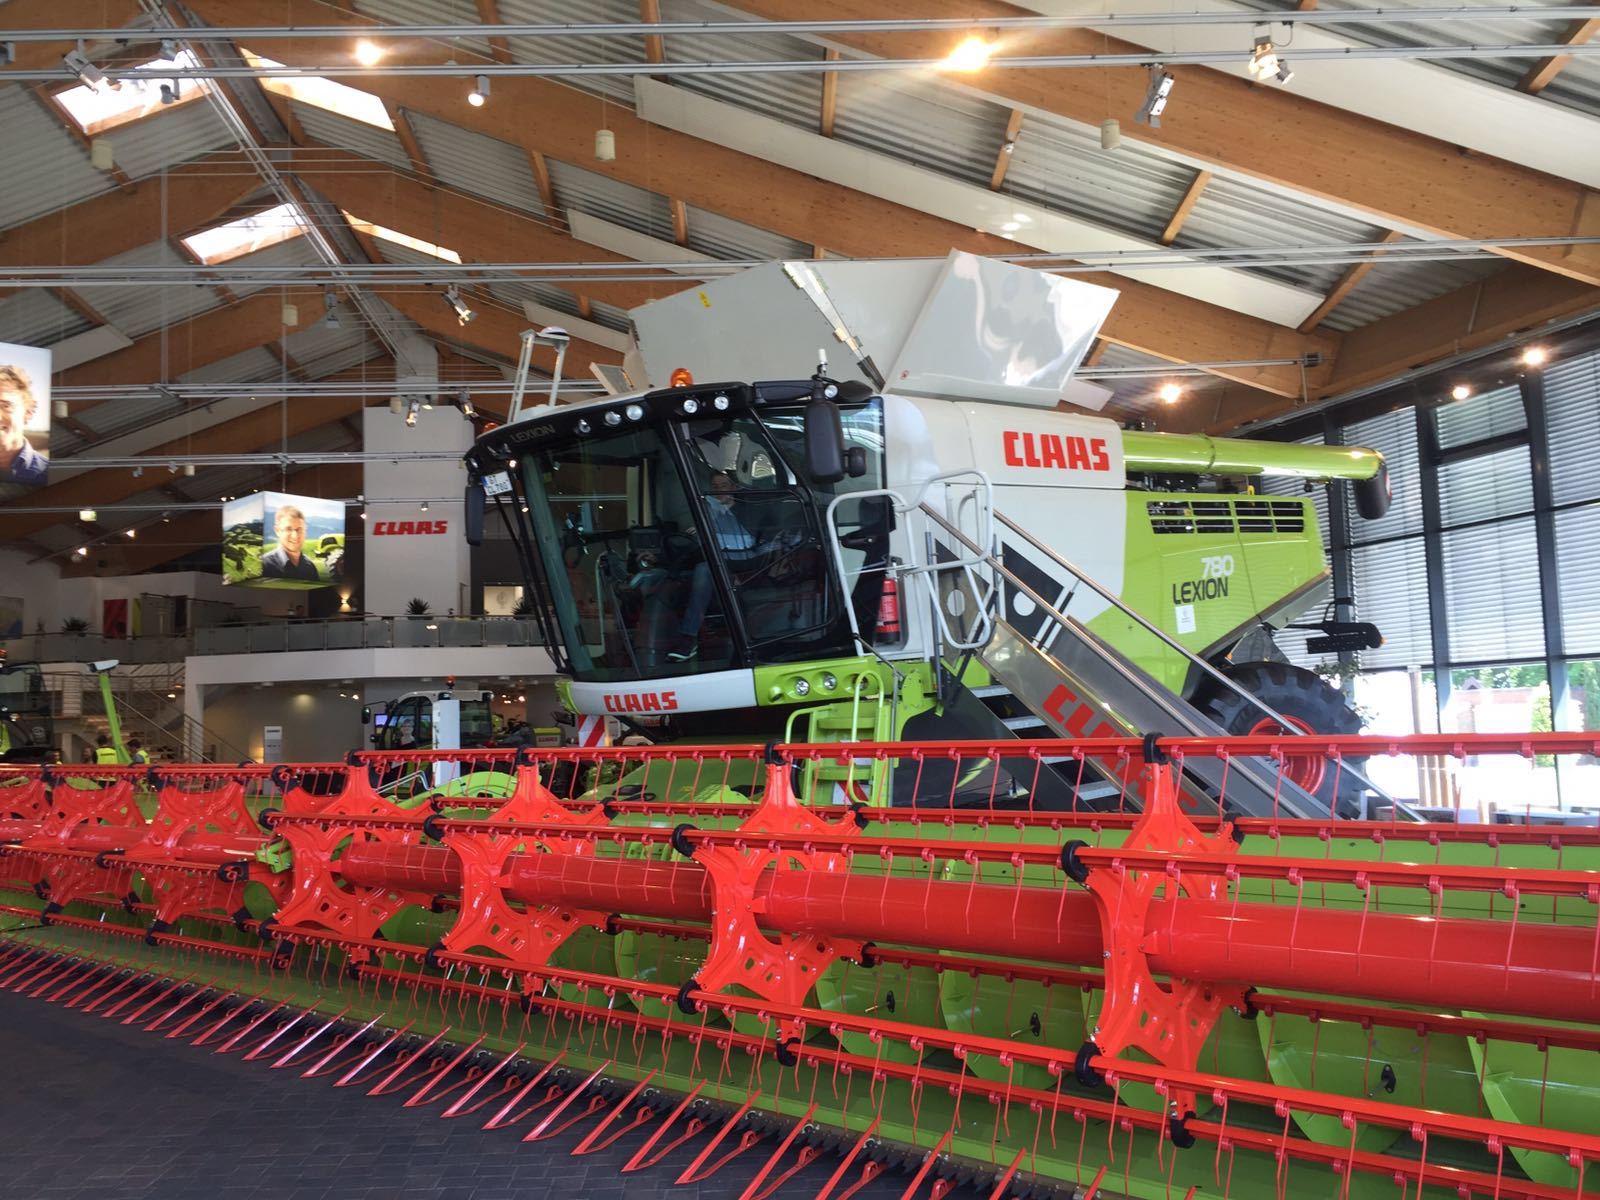
\includegraphics[width=\linewidth]{lexion.jpg}
    \end{textblock*}%

    \textbf{About Me}
    \begin{itemize}
        \item IRC-nick: CoLa
        \item KDE developer since $\approx$ 2010
        \item did PhD in algorithmic game theory\\ at Paderborn University \hspace{2.5cm}$\nearrow$
        \item now working as developer at CLAAS E-Systems in department for displays and operator panels for big agriculture machines
    \end{itemize}
    \bigskip

    \textbf{This talk is about the QtWayland Compositor Framework:}
    \begin{enumerate}
        \item topic is between my KDE and my professional work
        \item practical introduction how to create your own compositor
        \item the talk shall make you eager to experiment with the QtWaylandCompositor
        \item want to convince you that there is a new solution for many embedded device needs
    \end{enumerate}
\end{frame}

\usebackgroundtemplate{%
  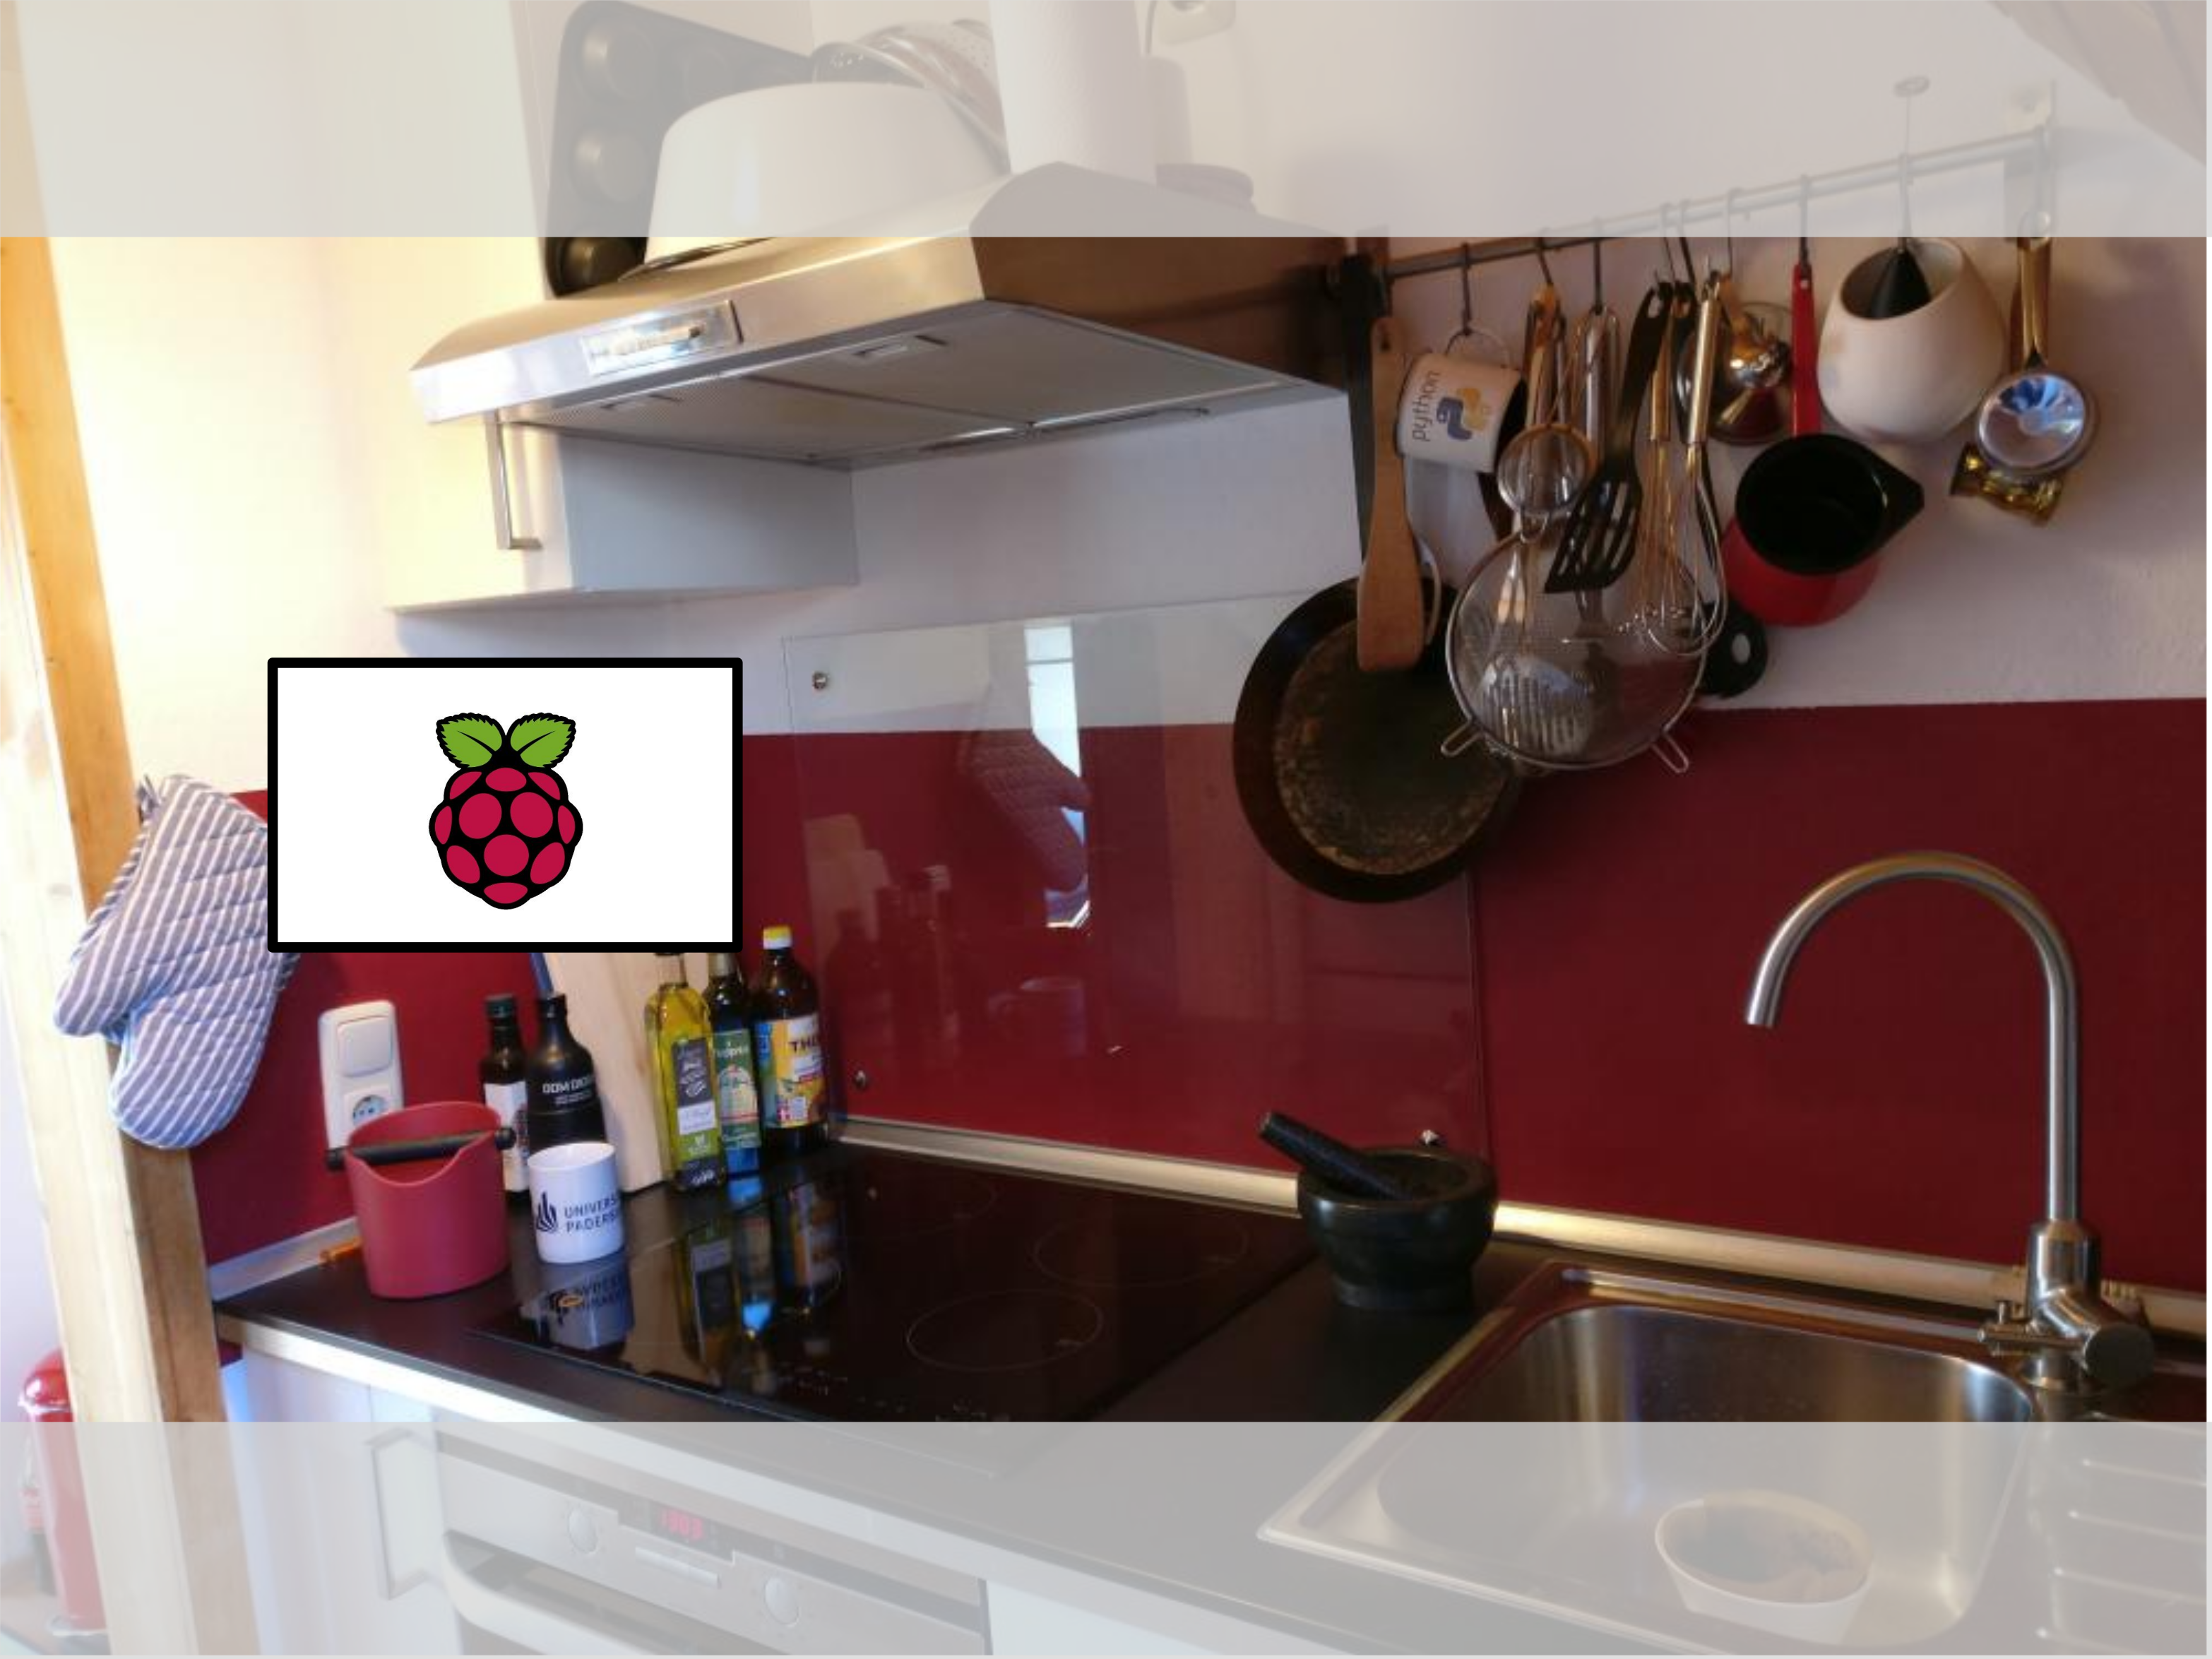
\includegraphics[width=\paperwidth,height=\paperheight]{kitchen-device.png}}

\begin{frame}
    {The Red Thread}
    {Let's say, I need a terminal for helping me in the kitchen\dots}
\end{frame}
\usebackgroundtemplate{}

\begin{frame}
    {Setting \& Requirements}

    \begin{textblock*}{.4\paperwidth}[1,0](\paperwidth,0pt)%
        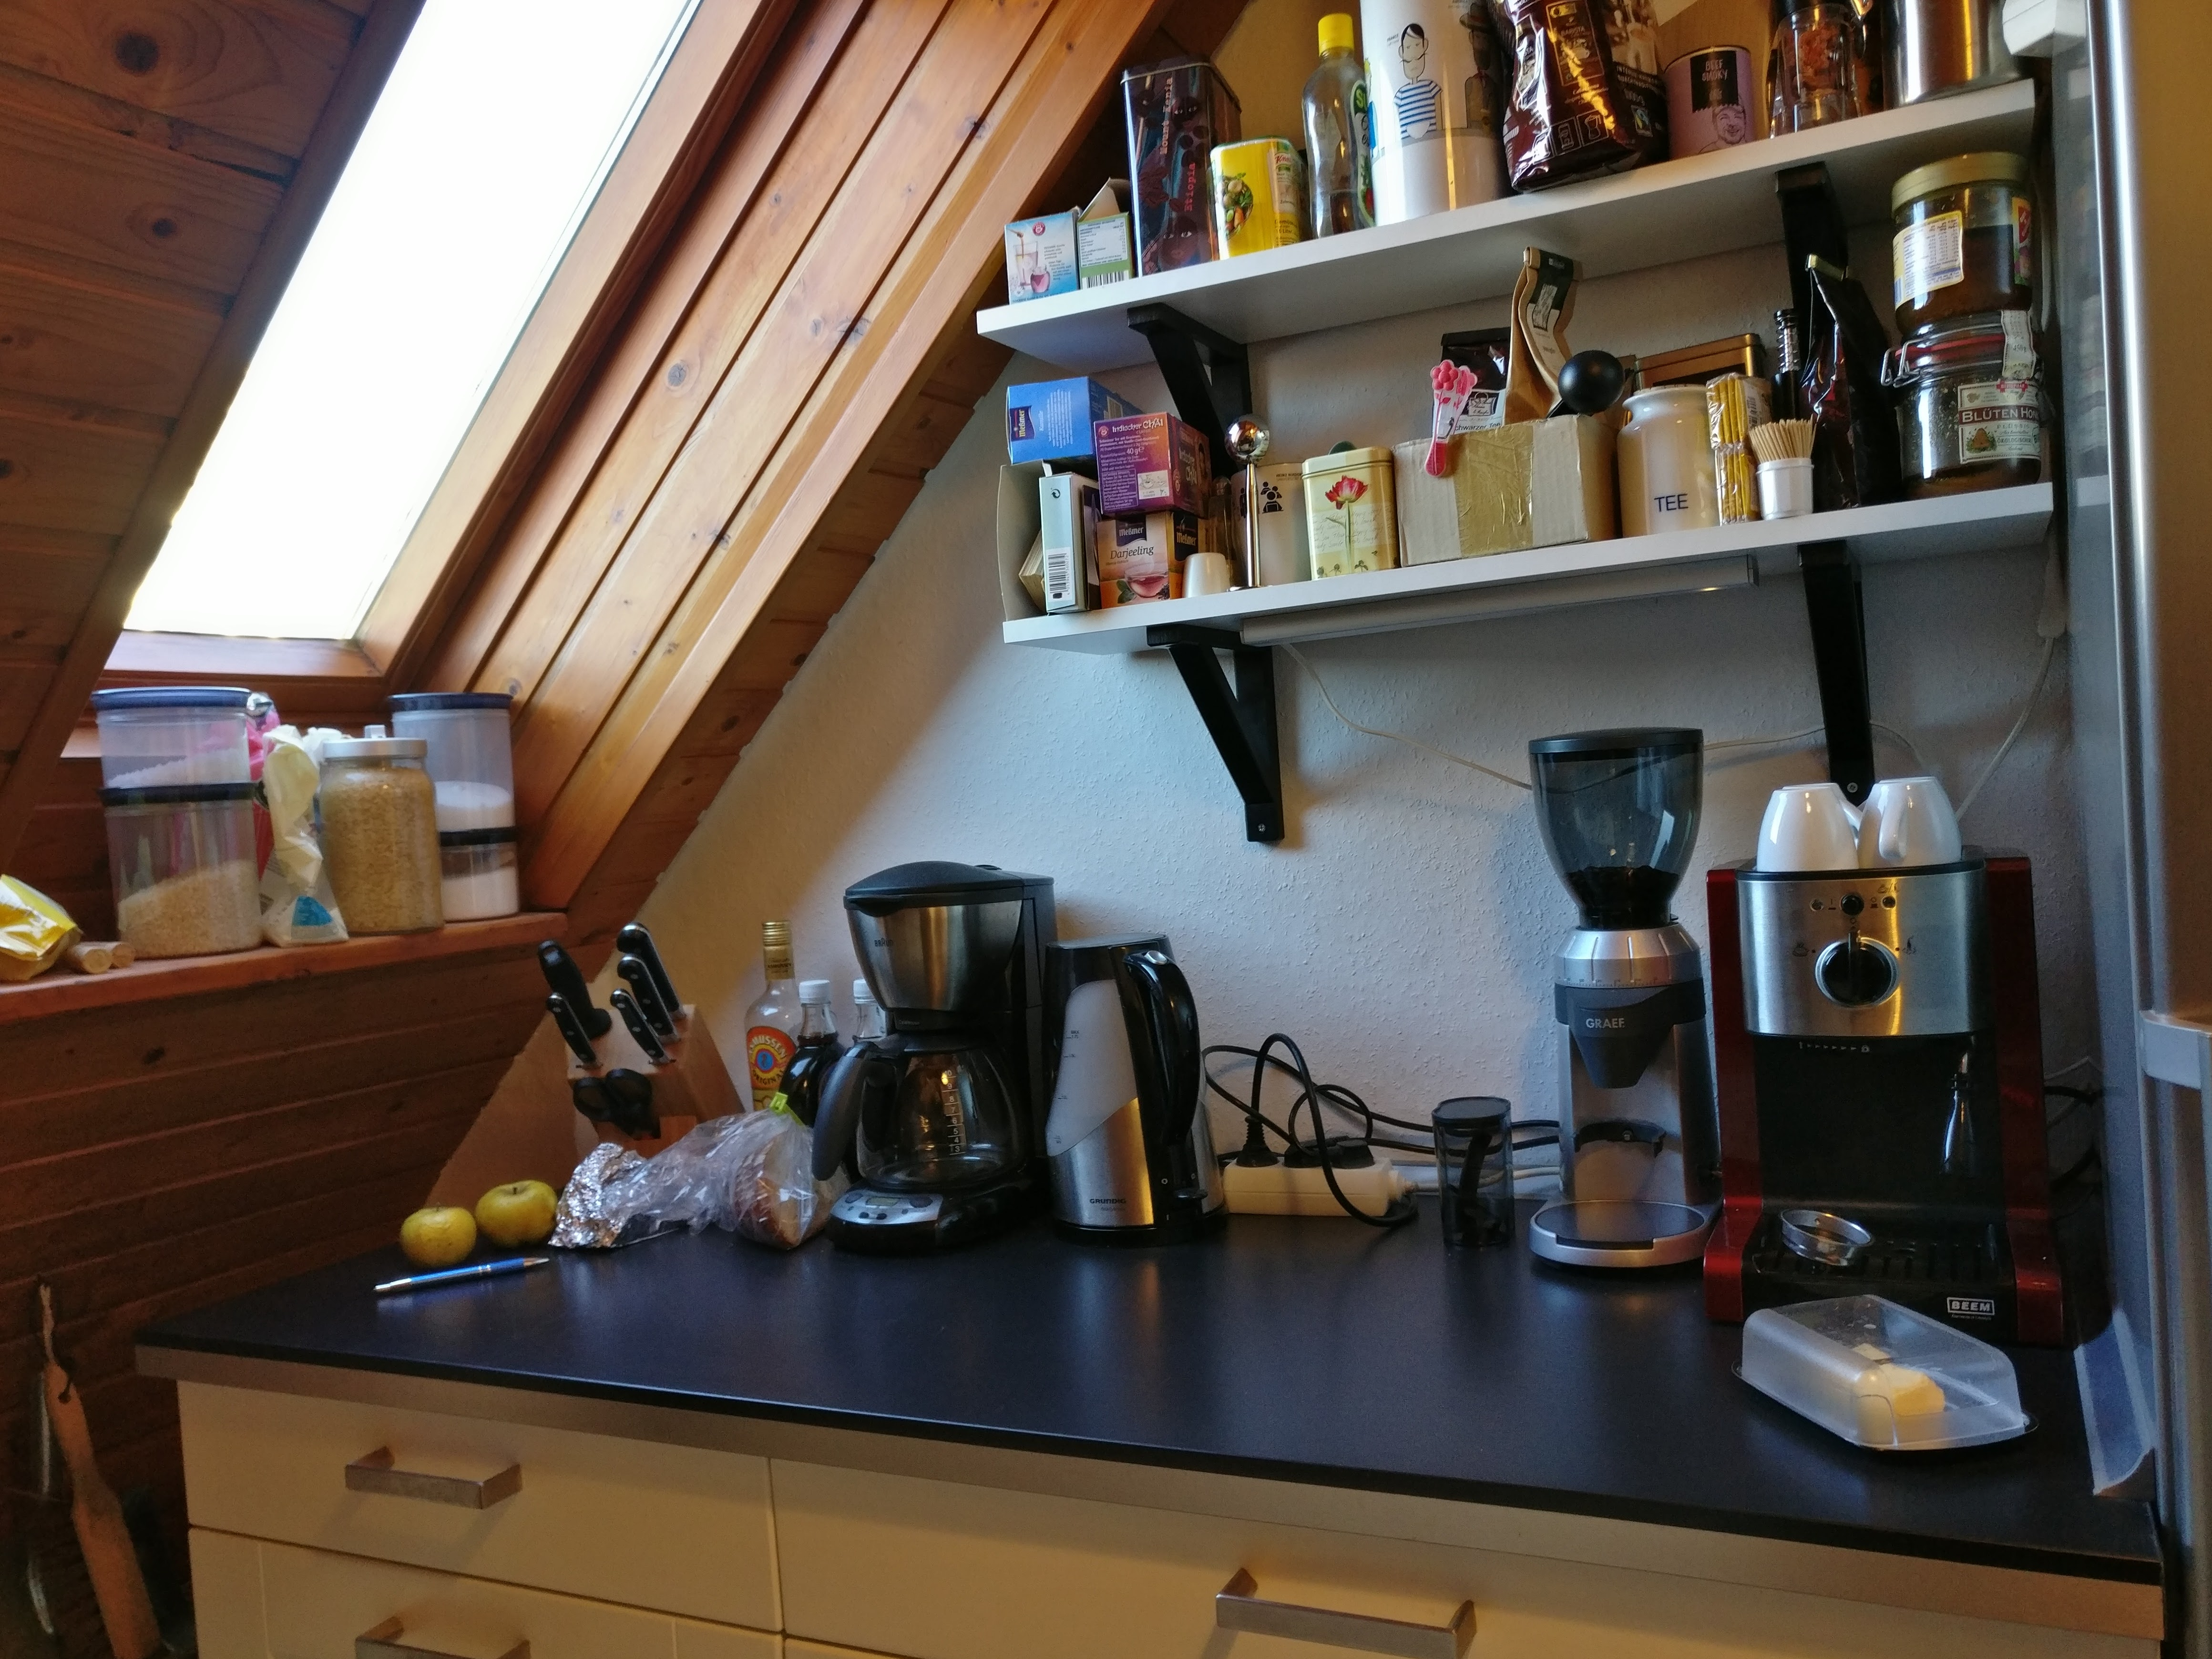
\includegraphics[width=\linewidth]{kitchen-right.jpg}
    \end{textblock*}%

    \begin{itemize}
        \item several applications shall run on the device
            \begin{itemize}
                \item cooking eggs timer app
                \item tea timer app
                \item current time app
            \end{itemize}
        \item seemless UI between the application windows
        \item swipe animation for switching applications
        \item want to use a standard embedded Linux based device with\\
            3D acceleration (e.g. Raspberry Pi)
    \end{itemize}

    \begin{itemize}
        \item [$\rightarrow$] we need a (Wayland) compositor
        \item [$\rightarrow$] we can use QtQuick
    \end{itemize}
    \vfill

    \emph{Yes, the above can be achieved in a much simpler way, but by exchanging these trivial apps with eg.\ internet radio, navigation system etc.\ and you get exactly what modern cars put onto their devices today.}
\end{frame}

\begin{frame}
    {Interaction Concept for the Kitchen Device}
    {Something your designer might come up with}

    \begin{center}
        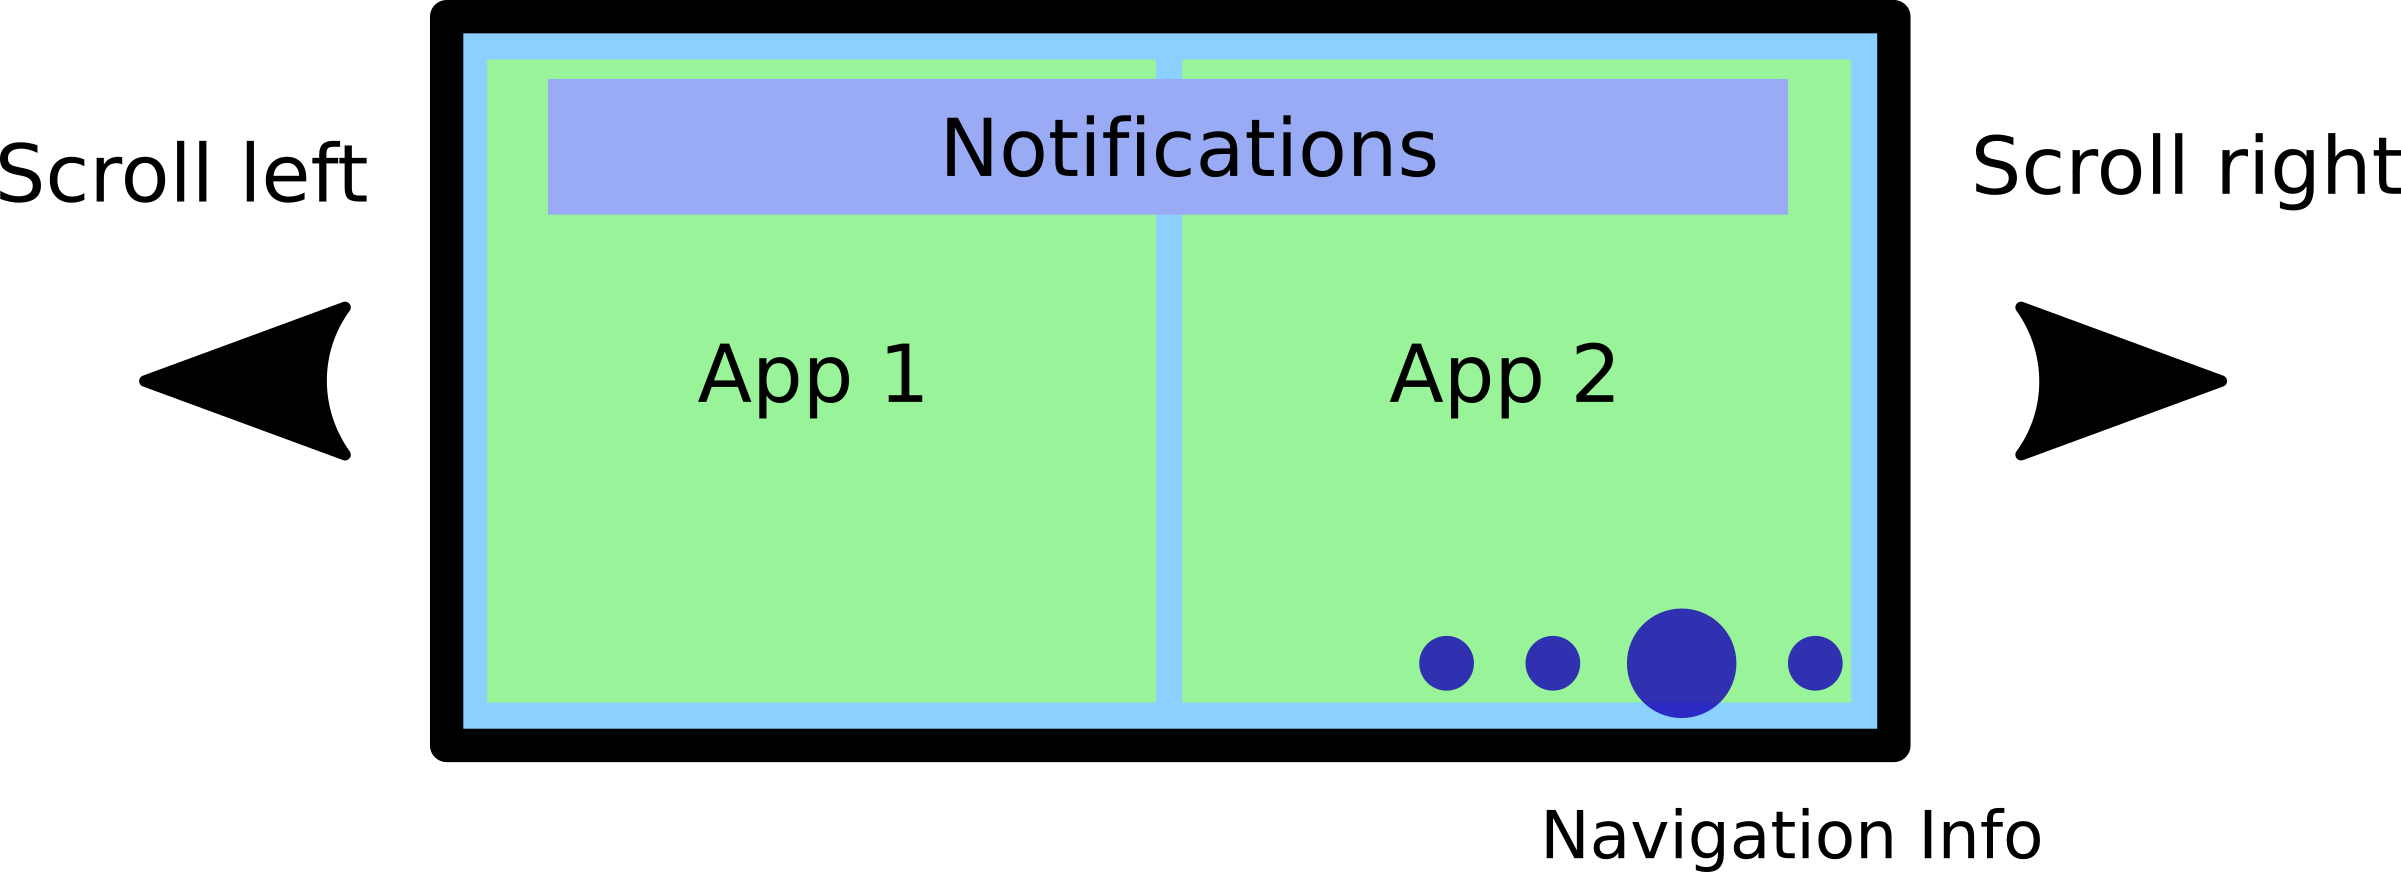
\includegraphics[width=.8\paperwidth]{interactionconcept.png}
    \end{center}
    \bigskip

    The remainder of the talk: how QtWayland helps to build this
\end{frame}

\begin{frame}
    {What is Wayland, again?}
    {A much too short answer for this question.}

    \begin{textblock*}{.2\paperwidth}[1,0](0.95\paperwidth,.05\paperheight)%
        
\includegraphics[width=\linewidth]{wayland.png}
    \end{textblock*}%

    Wayland is a protocol specifying the communication between\\
    a compositor (display server) and its clients (applications with\\
    their windows)

    \begin{itemize}
        \item in the embedded world, Wayland is the already established successor of X
        \item there are several Wayland compositor implementations:
            \begin{itemize}
                \item Weston: the reference implementation
                \item for desktop environments: KWin, Mutter, Enlightment \dots
                \item some propriatary compositors by device vendors exist
            \end{itemize}
        \item protocol extensions add further functionaly to the Wayland protocol:
            \begin{itemize}
                \item specified in XML files, code generated via wayland-scanner
            \end{itemize}
        \item available shells:
            \begin{itemize}
                \item [wl-shell] default protocol for window handling, already introduced with Wayland 1.0
                \item [xdg-shell] successor of wl\_shell with implementations provided by individual compositors
                \item [ivi-shell] protocol specifically for special automative form factors  (IVI = in-vehicle infotainment), used via the ivi-controller protocol extension
            \end{itemize}
    \end{itemize}
\end{frame}

\begin{frame}
    {The Qt Wayland Compositer API}

    \url{http://doc.qt.io/qt-5/qtwaylandcompositor-index.html}

    \begin{itemize}
        \item possible to write a compositor in just QML\\
            $\rightarrow$ QML is declarative language especially used for UI development on embedded devices/smartphones/touch applications
        \item supports Qt/C++ wrapper generation for Wayland protocol extensions
        \item supports multiple screen outputs
        \item provides wl-shell, xdg-shell and ivi-shell protocols
        \item History:
            \begin{itemize}
                \item since many years, there was an internal (but cumbersome to use) API
                \item Compositor API rewritten for Qt 5.7 (tech preview)
                \item Stable API since Qt 5.8 \alert{check if release happened until today :)}
            \end{itemize}
    \end{itemize}
    \medskip

    \textbf{Alternatives:} What about using the IVI-Shell extension in kitchen scenario?
    \begin{itemize}
        \item protocol only suited for very static settings
        \item touch gestures and window animations hard to implement
    \end{itemize}
\end{frame}

\begin{frame}
    {Possible System Architectures for my Kitchen Device}

    \textbf{Components:}
    \begin{description}
        \item [apps] Qt application running as Wayland client (with Qt: running on Wayland QPA with {\tt -platform wayland})
        \item [compositor] application acting as Wayland Server
        \item [shell] (optional, but IMO very reasonable) application that handles the more complex compositing logic and encapsulates all Wayland communication; eg. filters and sorts all safety relvant notifications from your applications
    \end{description}
    \medskip

    \begin{multicols}{2}
        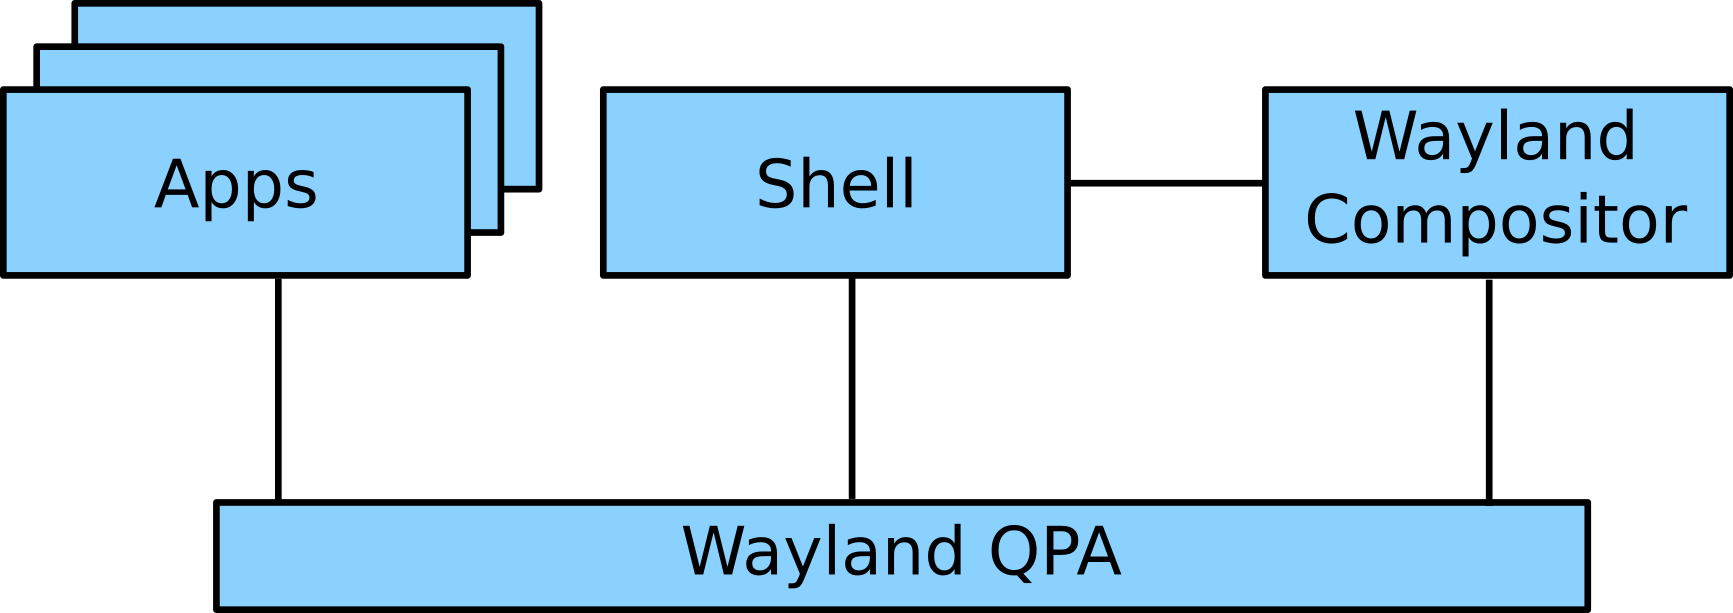
\includegraphics[width=\linewidth]{architecture.png}
        \columnbreak

        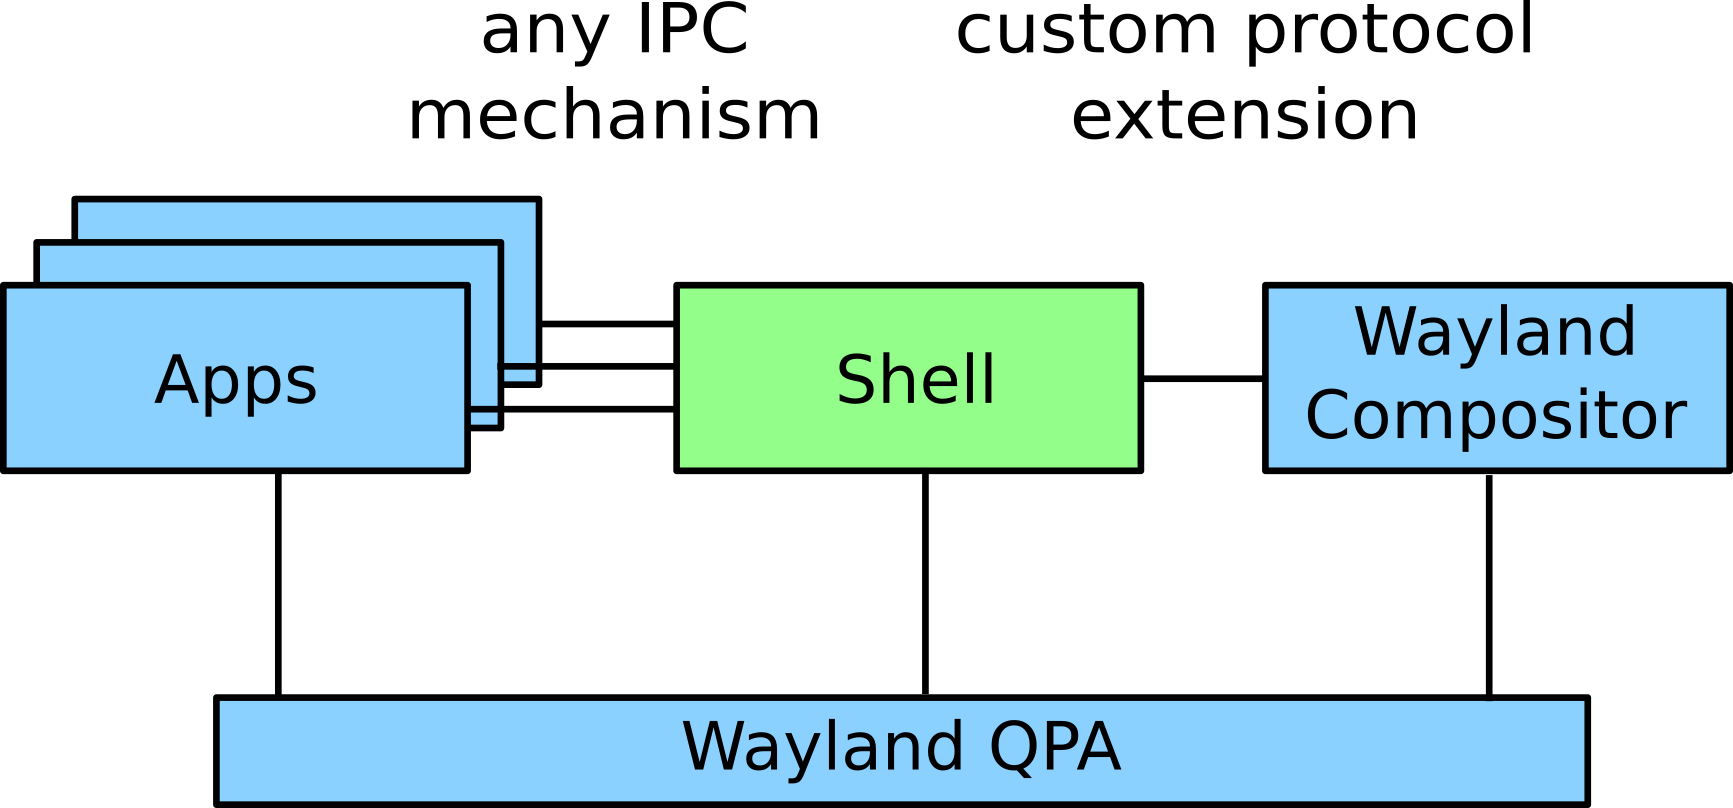
\includegraphics[width=\linewidth]{architecture-shell.png}
    \end{multicols}

    Note: in this talk I will stick to the left variant
\end{frame}

\begin{frame}
    {One-Slide Wayland Compositor}
    \vspace{-1em}
    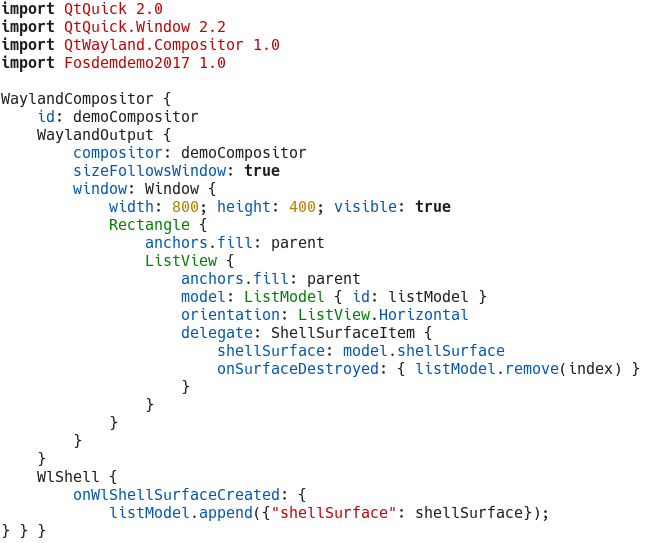
\includegraphics[height=.8\paperheight]{OneSlideCompositor.png}
\end{frame}

\begin{frame}[fragile]
    {Essential Components (1/2)}
    {The Compositor and the Shell}

    \vspace{-1em}
    \begin{lstlisting}
WaylandCompositor {
    WaylandOutput { ... }
    WlShell {
        onWlShellSurfaceCreated: {
            // handle shellSurface object
            listModel.append({"shellSurface": shellSurface});
        }
    }
}
    \end{lstlisting}
    \vspace{-1em}

    \textbf{WaylandCompositor}
    \begin{itemize}
        \item representation of the compositor
        \item usually the root object of the scene
        \item always should have output and shell extension
    \end{itemize}
    \smallskip

    \textbf{Shell Extension}
    \begin{itemize}
        \item the protocol interface that gives access to the surfaces
        \item WlShell and XdgShell are supported
        \item handle the \texttt{onWlSurfaceCreated()} signal
    \end{itemize}
\end{frame}

\begin{frame}[fragile]
    {Essential Components (2/2)}
    {The Surface Items and the Output}

    \vspace{-1em}
    \begin{lstlisting}
WaylandOutput {
    compositor: demoCompositor
    sizeFollowsWindow: true
    window: Window {
        width: 800; height: 400; visible: true
        ListView {
            anchors.fill: parent
            model: ListModel { id: listModel }
            orientation: ListView.Horizontal
            delegate: ShellSurfaceItem {
                shellSurface: model.shellSurface
                onSurfaceDestroyed: { listModel.remove(index) }
}   }   }   }
    \end{lstlisting}
    \vspace{-1em}

    \textbf{ShellSurfaceItem and QWaylandQuickItem}
    \begin{itemize}
        \item wrapper around shell surfaces to handle them like ordinary QtQuick Items
        \item visibility and input behavior follows typical QtQuick mechanisms
    \end{itemize}
    \smallskip

    \textbf{Output}
    \begin{itemize}
        \item manages rectangular output region in which content can be shown
        \item compositor can have multiple outputs
    \end{itemize}
\end{frame}


\begin{frame}[fragile]
    {Protocol Extension for Alarm Notifications (1/2)}
    {How to add your own custom Wayland protocol?}

    \textbf{Code:}\ {\small \url{https://github.com/cordlandwehr/fosdem-2017-talk-qtwayland/tree/master/demo}}
    \bigskip

    \textbf{The Custom Protocol Extension}
\begin{lstlisting}[language=Xml]
<protocol>
    <interface name="demo_extension" version="1">

        <request name="notification">
          <description summary="Example Notification Event">
            Example request from client to server
          </description>

          <arg name="text" type="string"/>
        </request>
    </interface>
</protocol>
\end{lstlisting}
\end{frame}

\begin{frame}[fragile]
    {Protocol Extension for Alarm Notifications (2/2)}
    {How to add your own custom Wayland protocol?}

    \textbf{On the Compositor Side}
    \begin{enumerate}
        \item create QWaylandCompositorExtensionTemplate derived protocol wrapper
        \item use qtwayland-scanner to generate Qt \& C++ binding classes for protocol
        \item add CustomExtension in the WaylandCompositor element in the QtQuick context and connect to signals/use methods for sending data
    \end{enumerate}
    \bigskip

    \textbf{On the Client (Application) Side}
    \begin{enumerate}
        \item create QWaylandClientExtensionTemplate derived protocol wrapper
        \item use qtwayland-scanner to generate Qt \& C++ binding classes for protocol
        \item create client protocol wrapper instance and use it
    \end{enumerate}

\end{frame}

\begin{frame}
    {Demo}
    {Everything put together with some QtQuick UI sugar.}

    \begin{center}
        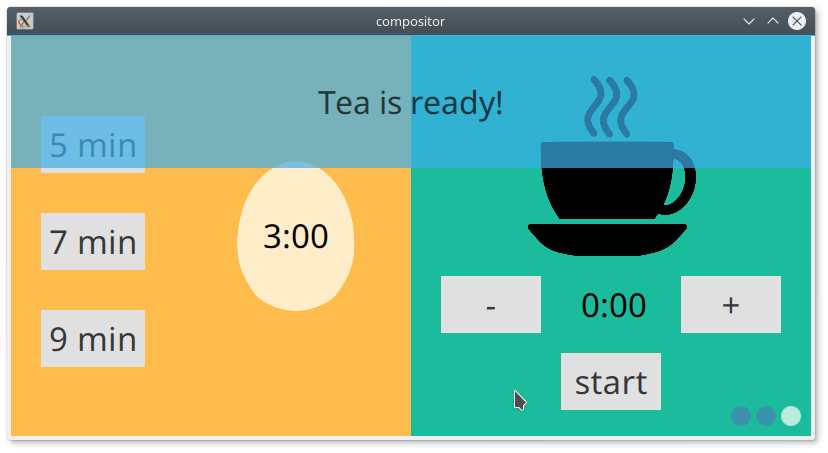
\includegraphics[width=\linewidth]{demo_screenshot.png}
    \end{center}
\end{frame}

\begin{frame}
    {Conclusion}

    \begin{itemize}
        \item the QtWayland Compositor framework drastically simplifies the creation of a compositor for a specific/special UX requirement
        \item prototyping such a compositor is just a matter of a day
        \item window compositing becomes UI design:
            \begin{itemize}
                \item when a surface looks and behaves like a QtQuick item, you can handle it like a QtQuick item\dots
                \item no special Wayland developer needed but ``just'' a QtQuick UI developer can develop your compositor tailored for your individual form factor
            \end{itemize}
        \item [$\rightarrow$] try it out!
    \end{itemize}
    \vfill
    Demo and all sources of this talk are available here:\\
    {\small \url{https://github.com/cordlandwehr/fosdem-2017-talk-qtwayland/tree/master/demo}}
\end{frame}

\begin{frame}
    {References}

    \begin{itemize}
        \item Johan's ``The Qt Wayland Compositor API'' introduction talk at QtCon 2016\\
            \url{https://conf.qtcon.org/en/qtcon/public/events/392}
        \item Online Help\\
            \url{http://doc.qt.io/qt-5/qtwaylandcompositor-index.html}
        \item IRC at freenode: \#qt-lighthouse
    \end{itemize}
\end{frame}

\KDElastframe

\end{document}
